\documentclass[12pt, a4paper, oneside]{ctexart}
\usepackage{amsmath, amsthm, amssymb, bm, graphicx, hyperref, mathrsfs}

\title{\textbf{Homework}}
\author{PB22010344 黄境}
\date{\today}
\linespread{1.5}
\newcounter{exercisename}
\newenvironment{exercise}{\stepcounter{exercisename}\par\noindent\textsc{Exercise \arabic{exercisename}. }}{\\\par}
\newenvironment{solution}{\par\noindent\textsc{Solution. }}{\\\par}
\newenvironment{note}{\par\noindent\textsc{Note of Problem \arabic{exercisename}. }}{\\\par}

\DeclareMathOperator*{\argmin}{\bf argmin}
\newcommand{\proj}[2]{\textbf{P}_{#2} (#1)}
\newcommand{\lspan}[1]{\textbf{span}  (#1)  }
\newcommand{\rank}[1]{ \textbf{rank}  (#1)  }
\newcommand{\RNum}[1]{\uppercase\expandafter{\romannumeral #1\relax}}
\DeclareMathOperator*{\cl}{\bf cl\,}
\DeclareMathOperator*{\bd}{\bf bd\,}
\DeclareMathOperator*{\conv}{\bf conv\,}
\DeclareMathOperator*{\epi}{\bf epi\,}

\begin{document}

\maketitle

\begin{exercise}
    \bf Projection
\end{exercise}

\begin{solution}
	1. Suppose that $\exists \mathbf{z}_{1} \neq \mathbf{z}_{2}$, such that
	$\mathbf{z}_{1} = \mathbf{z}_{2} = \text{proj}_{\mathbf{A}}(\mathbf{x})$. 
	Since $\mathbf{z}_{1}, \mathbf{z}_{2} \in \mathcal{C}(\mathbf{A})$, we have 
	\[
	\frac{\mathbf{z}_{1} + \mathbf{z}_{2}}{2} \in \mathcal{C}(\mathbf{A}), \quad \frac{\mathbf{z}_{1} + \mathbf{z}_{2}}{2} \neq \mathbf{z}_{1}, \quad \frac{\mathbf{z}_{1} + \mathbf{z}_{2}}{2} \neq \mathbf{z}_{2}.
	\]
	Since the norm satisfies the Triangle Inequality, we have
	\[
	\left\| \mathbf{x} - \frac{\mathbf{z}_{1} + \mathbf{z}_{2}}{2} \right\| = \frac{\| (\mathbf{x} - \mathbf{z}_{1}) + (\mathbf{x} - \mathbf{z}_{2}) \|}{2}
	< \frac{\|\mathbf{x} - \mathbf{z}_{1}\| + \|\mathbf{x} - \mathbf{z}_{2}\|}{2} = \|\mathbf{x} - \mathbf{z}_{1}\|,
	\]
	which contradicts the assumption that $\|\mathbf{x} - \mathbf{z}_{1}\|$ is the smallest for all $\mathbf{z} \in \mathcal{C}(\mathbf{A})$.
	Thus, the projection $\text{proj}_{\mathbf{A}}(\mathbf{x})$ must be unique. 
	\newline\newline
	2.(a) In fact, the subspace generated by $\mathbf{v}_i$ is given by
	\[
	\{\alpha \mathbf{v}_{i} : \alpha \in \mathbb{R}\}.
	\]
	Thus, the projection of $\mathbf{w}$ onto $\mathbf{v}_1$ is
	\[
	\proj{\mathbf{w}}{\mathbf{v}_1} = \arg\min\limits_{\alpha\mathbf{v}_1} \left\{ \|\mathbf{w} - \alpha \mathbf{v}_1\| : \alpha \in \mathbb{R} \right\}.
	\]
	Since
	\[
	\|\mathbf{w} - \alpha \mathbf{v}_1\|^2 = (\mathbf{w} - \alpha \mathbf{v}_1, \mathbf{w} - \alpha \mathbf{v}_1) = \alpha^2 \|\mathbf{v}_1\|^2 - 2 \alpha (\mathbf{w}, \mathbf{v}_1) + \|\mathbf{w}\|^2,
	\]
	we see that this is a quadratic function of $\alpha$. Minimizing it gives
	\[
	\arg\min\limits_{\alpha} \|\mathbf{w} - \alpha \mathbf{v}_1\|^2 = \frac{-2 (\mathbf{w}, \mathbf{v}_1)}{-2 \|\mathbf{v}_1\|^2} = \frac{(\mathbf{w}, \mathbf{v}_1)}{\|\mathbf{v}_1\|^2}.
	\]
	Thus, the projection is
	\[
	\proj{\mathbf{w}}{\mathbf{v}_1} = \frac{(\mathbf{w}, \mathbf{v}_1)}{\|\mathbf{v}_1\|^2} \mathbf{v}_1.
	\]
	\newline\newline
    (b) Since the inner product is bilinear, we have 
    \[
    \proj{\alpha \mathbf{u} + \beta \mathbf{w}}{\mathbf{v}_1} = \frac{(\alpha \mathbf{u} + \beta \mathbf{w}, \mathbf{v}_1)}{\|\mathbf{v}_1\|^2} \mathbf{v}_1
    = \frac{(\alpha \mathbf{u}, \mathbf{v}_1) + (\beta \mathbf{w}, \mathbf{v}_1)}{\|\mathbf{v}_1\|^2} \mathbf{v}_1
    \]
    \[
    = \alpha \frac{(\mathbf{u}, \mathbf{v}_1)}{\|\mathbf{v}_1\|^2} \mathbf{v}_1 + \beta \frac{(\mathbf{w}, \mathbf{v}_1)}{\|\mathbf{v}_1\|^2} \mathbf{v}_1
    = \alpha \proj{\mathbf{u}}{\mathbf{v}_1} + \beta \proj{\mathbf{w}}{\mathbf{v}_1}.
    \]
    \newline\newline
    (c) Since $(\mathbf{a}, \mathbf{b}) = \mathbf{a}^T \mathbf{b}$, we have
    \[
    \proj{\mathbf{w}}{\mathbf{v}_1} = \frac{(\mathbf{v}_1, \mathbf{w})}{\|\mathbf{v}_1\|^2} \mathbf{v}_1 = \mathbf{v}_1 \frac{\mathbf{v}_1^T \mathbf{w}}{\|\mathbf{v}_1\|^2},
    \]
    which implies
    \[
    \mathbf{H} = \frac{\mathbf{v}_1 \mathbf{v}_1^T}{\|\mathbf{v}_1\|^2}.
    \]
    \newline\newline
    (d)(i) Firstly, we will prove that if $(\mathbf{w} - \mathbf{z}, \mathbf{x}) = 0$, $\forall\, \mathbf{x} \in \mathcal{C}(\mathbf{V})$, then $\mathbf{z}$ must be $\proj{\mathbf{w}}{\mathbf{V}}$. Since 
    \[
    \mathcal{C}(\mathbf{V}) = \{\mathbf{x} \in \mathbb{R}^{n \times 1}: \mathbf{x} = \mathbf{V} \mathbf{a}, \mathbf{a} \in \mathbb{R}^{d \times 1}\}, \forall\, \mathbf{x} \neq \mathbf{z}\, \text{and}\, \mathbf{x} \in \mathcal{C}(\mathbf{V}),
    \]
    we can find $\mathbf{a}_0 \neq \mathbf{0}$ such that $\mathbf{x} = \mathbf{z} + \mathbf{V} \mathbf{a}_0$. Therefore,
    \[
    \|\mathbf{w} - \mathbf{x}\|^2 = (\mathbf{w} - \mathbf{x}, \mathbf{w} - \mathbf{x}) = (\mathbf{w} - \mathbf{z} - \mathbf{V} \mathbf{a}_0, \mathbf{w} - \mathbf{z} - \mathbf{V} \mathbf{a}_0) 
    \]
    \[
    = \|\mathbf{w} - \mathbf{z}\|^2 + \|\mathbf{V} \mathbf{a}_0\|^2 - 2 (\mathbf{w} - \mathbf{z}, \mathbf{V} \mathbf{a}_0).
    \]
    Since $\mathbf{V} \mathbf{a}_0 \in \mathcal{C}(\mathbf{V})$ and  $\mathbf{a}_0 \neq \mathbf{0}$, 
    we have 
    \[
    \|\mathbf{w} - \mathbf{x}\|^2 = \|\mathbf{w} - \mathbf{z}\|^2 + \|\mathbf{V} \mathbf{a}_0\|^2 \geq \|\mathbf{w} - \mathbf{z}\|^2, \forall\, \mathbf{x} \in \mathcal{C}(\mathbf{V}),
    \]
    which implies $\mathbf{z} = \proj{\mathbf{w}}{\mathbf{V}}$. 
    Since 
    \[
    (\mathbf{w} - \mathbf{z}, \mathbf{x}) = 0, \forall\, \mathbf{x} \in \mathcal{C}(\mathbf{V}) \Leftrightarrow (\mathbf{w} - \mathbf{z}, \mathbf{v}_i) = 0, \forall\, \mathbf{v}_i \Leftrightarrow \mathbf{V}^T (\mathbf{w} - \mathbf{z}) = \mathbf{0},
    \]
    let $\mathbf{z} = \mathbf{V} \mathbf{x}_0$, then $\mathbf{V}^T \mathbf{w} = \mathbf{V}^T \mathbf{z} = \mathbf{V}^T \mathbf{V} \mathbf{x}_0$. Since $\mathbf{v}_i$ are linearly independent, $\mathbf{V}^T \mathbf{V}$ is invertible. Thus
    \[
    \mathbf{x}_0 = (\mathbf{V}^T \mathbf{V})^{-1} \mathbf{V}^T \mathbf{w} \Rightarrow \proj{\mathbf{w}}{\mathbf{V}} = \mathbf{z} = \mathbf{V} \mathbf{x}_0 = \mathbf{V} (\mathbf{V}^T \mathbf{V})^{-1} \mathbf{V}^T \mathbf{w},
    \]
    and
    \[
    \mathbf{H} = \mathbf{V} (\mathbf{V}^T \mathbf{V})^{-1} \mathbf{V}^T.
    \]
    \newline\newline
    (ii) Since $\mathbf{v}_i^T \mathbf{v}_j = 0$, for all $i \neq j$, we notice that $\mathbf{V}^T \mathbf{V} = \text{diag}(\|\mathbf{v}_1\|^2, \|\mathbf{v}_2\|^2, \dots, \|\mathbf{v}_d\|^2)$, and thus 
    \[
    (\mathbf{V}^T \mathbf{V})^{-1} = \text{diag}(\|\mathbf{v}_1\|^{-2}, \|\mathbf{v}_2\|^{-2}, \dots, \|\mathbf{v}_d\|^{-2}).
    \]
    Therefore, we have
    \[
    \mathbf{H} = \mathbf{V} \text{diag}(\|\mathbf{v}_1\|^{-2}, \|\mathbf{v}_2\|^{-2}, \dots, \|\mathbf{v}_d\|^{-2}) \mathbf{V}^T = \text{diag}\left( \frac{\mathbf{v}_1}{\|\mathbf{v}_1\|^2}, \frac{\mathbf{v}_2}{\|\mathbf{v}_2\|^2}, \dots, \frac{\mathbf{v}_n}{\|\mathbf{v}_n\|^2} \right) \mathbf{V}^T
    \]
    \[
    = \text{diag}(\mathbf{v}_1 \mathbf{v}_1^T \|\mathbf{v}_1\|^{-2}, \mathbf{v}_2 \mathbf{v}_2^T \|\mathbf{v}_2\|^{-2}, \dots, \mathbf{v}_d \mathbf{v}_d^T \|\mathbf{v}_d\|^{-2}).
    \]
    \newline\newline
    3. (a) Since $\mathbf{A} = \mathbf{I}_{2}$, we have $\mathbf{Ax} = \mathbf{x}$, $\forall\, \mathbf{x} \in \mathbb{R}^{2 \times 1}$, which also implies that $\mathbf{x} \in \mathcal{C}(\mathbf{A})$. Therefore, 
    \[
    \proj{\mathbf{x}}{\mathbf{A}} = \mathbf{x}, \forall\, \mathbf{x} \in \mathbb{R}^{2 \times 1},
    \]
    and the coordinates of $\proj{\mathbf{x}}{\mathbf{A}}$ are $(x_{1}, x_{2}) = \mathbf{x}$. Obviously, it's unique.
    \newline\newline
    (b) Let $\mathbf{x} = (x_{1}, x_{2})$. Consider $\mathcal{C}(\mathbf{A})$, suppose that $\mathbf{y} \in \mathcal{C}(\mathbf{A})$, $\mathbf{y} = \mathbf{Az}$ and $\mathbf{z = (z_{1}, z_{2})^{T}}$. Therefore, 
    \[
    \mathbf{y} = \mathbf{A}((z_{1}, z_{2})^{T}) = (z_{1} + 2z_{2}, z_{1} + 2z_{2})^{T},
    \]
    which implies 
    \[
    \mathcal{C}(\mathbf{A}) = \{a(1, 1)^{T}: a \in \mathbb{R}\}.
    \]
    From the conclusion in exercise 1.2(a), we have
    \[
    \proj{\mathbf{x}}{\mathbf{A}} = \frac{(\mathbf{w}, \mathbf{v}_{1})}{\|\mathbf{v}_{1}\|^{2}}\mathbf{v}_{1} = \frac{x_{1} + x_{2}}{2}(1, 1) = \left( \frac{x_{1} + x_{2}}{2}, \frac{x_{1} + x_{2}}{2} \right).
    \]
    Also, it's unique.
\end{solution}
	
\begin{exercise}
	\bf Projection to a Matrix Space
\end{exercise}

\begin{solution}
	1. Suppose that $\mathbf{A} = \text{diag}(a_{1}, a_{2}, \dots, a_{n})$, $\mathbf{B} = \text{diag}(b_{1}, b_{2}, \dots, b_{n}) \in \mathbb{R}^{n \times n}$ are diagonal matrices and $\alpha$, $\beta \in \mathbb{R}$. We have 
	\[
	\alpha\mathbf{A} + \beta\mathbf{B} = \text{diag}(\alpha a_{1} + \beta b_{1}, \alpha a_{2} + \beta b_{2}, \dots, \alpha a_{n} + \beta b_{n}),
	\]
	which is also a diagonal matrix. Thus, the set of diagonal matrices in $\mathbb{R}^{n \times n}$ forms a linear space. Since the inner product is $(\mathbf{A}, \mathbf{B}) = \text{tr}(\mathbf{A}^{T} \mathbf{B})$, the norm is defined as
	\[
	\|\mathbf{A}\| = \sqrt{\text{tr}(\mathbf{A}^{T} \mathbf{A})} = \sqrt{\sum_{i=1}^{n} \sum_{j=1}^{n} a_{ij}^{2}}.
	\]
	Let $\mathbf{D} = \text{diag}(d_{1}, d_{2}, \dots, d_{n})$, therefore $\forall\, \mathbf{A} \in \mathbb{R}^{n \times n}$, we have
	\[
	\|\mathbf{A} - \mathbf{D}\|^{2} = \sum_{i=1}^{n} \sum_{j=1, j \neq i}^{n} a_{ij}^{2} + \sum_{i=1}^{n} (a_{ii} - d_{i})^{2}.
	\]
	By fixing all of the $d_{j}$ and taking the derivative of $d_{i}$, we can obtain that
	\[
	\min \|\mathbf{A} - \mathbf{D}\|^{2} = \sum_{j=1, j \neq i}^{n} a_{ij}^{2},
	\]
	and the equation holds if and only if $\mathbf{D} = \text{diag}(a_{11}, a_{22}, \dots, a_{nn})$. Thus, the projection of $\mathbf{A}$ onto the space of diagonal matrices is
	\[
	\mathbf{P(A)} = \text{diag}(a_{11}, a_{22}, \dots, a_{nn}).
	\]
	\newline\newline
	2. Suppose that $\mathbf{A}$, $\mathbf{B} \in \mathbb{R}^{n \times n}$ are symmetric matrices and $\alpha$, $\beta \in \mathbb{R}$. We have
	\[
	(\alpha \mathbf{A} + \beta \mathbf{B})^{T} = \alpha \mathbf{A}^{T} + \beta \mathbf{B}^{T} = \alpha \mathbf{A} + \beta \mathbf{B},
	\]
	which implies $\alpha \mathbf{A} + \beta \mathbf{B}$ is also a symmetric matrix. Thus, the set of symmetric matrices in $\mathbb{R}^{n \times n}$ forms a linear space $\mathbf{S}^{n \times n}$. Let $\mathbf{E}_{ij} = (e_{ij})_{n \times n}$, s.t. $e_{ij} = 1$ and $e_{ab} = 0, \forall a \neq i$ or $b \neq j$, then $\{\mathbf{E}_{ij} + \mathbf{E}_{ji}: 1 \leq i \leq j \leq n\}$ is a basis of $\mathbf{S}^{n \times n}$. Therefore, we have
	\[
	\text{dim}(\mathbf{S}^{n \times n}) = \binom{n}{2} = \frac{n(n + 1)}{2}.
	\]
	\newline\newline
	3. Suppose that $\mathbf{A}$ is symmetric and $\mathbf{B}$ is skew-symmetric. Since $\text{tr}(\mathbf{M}) = \text{tr}(\mathbf{M}^{T})$, $\forall\, \mathbf{M} \in \mathbb{R}^{n \times n}$, we have 
	\[
	(\mathbf{A}, \mathbf{B}) = \text{tr}(\mathbf{A}^{T}\mathbf{B}) = \text{tr}(\mathbf{A}\mathbf{B}) = \text{tr}((\mathbf{A}^{T}\mathbf{B})^{T}) = \text{tr}(\mathbf{B}^{T}\mathbf{A}) = -\text{tr}(\mathbf{B}\mathbf{A}) = -(\mathbf{B}, \mathbf{A}),
	\]
	which implies $(\mathbf{B}, \mathbf{A}) + (\mathbf{A}, \mathbf{B}) = 0$. Since the inner product is symmetric, we have $(\mathbf{B}, \mathbf{A}) = (\mathbf{A}, \mathbf{B})$, and therefore
	\[
	(\mathbf{B}, \mathbf{A}) + (\mathbf{A}, \mathbf{B}) = 2(\mathbf{A}, \mathbf{B}) = 0 \quad \Rightarrow \quad (\mathbf{A}, \mathbf{B}) = 0.
	\]
	Thus, the inner product between a symmetric and a skew-symmetric matrix is always zero.
	Now, suppose $\mathbf{A} \in \mathbb{R}^{n \times n}$. We can decompose $\mathbf{A}$ as follows:
	\[
	\mathbf{A} = \frac{\mathbf{A} + \mathbf{A}^{T}}{2} + \frac{\mathbf{A} - \mathbf{A}^{T}}{2}.
	\]
	Let $\mathbf{P} = \frac{\mathbf{A} + \mathbf{A}^{T}}{2}$ and $\mathbf{N} = \frac{\mathbf{A} - \mathbf{A}^{T}}{2}$. Clearly, $\mathbf{P} = \mathbf{P}^{T}$ and $\mathbf{N} = -\mathbf{N}^{T}$, which means that $\mathbf{P}$ is symmetric and $\mathbf{N}$ is skew-symmetric. Hence, $\mathbf{A} = \mathbf{P} + \mathbf{N}$, where $\mathbf{P}$ is symmetric and $\mathbf{N}$ is skew-symmetric.
	\newline\newline
	4. Suppose that $\mathbf{S} = (s_{ij}) \in \mathbb{R}^{n \times n}$ is a symmetric matrix and $\mathbf{A} = (a_{ij}) \in \mathbb{R}^{n \times n}$. The projection of $\mathbf{A}$ onto the space of symmetric matrices is obtained by minimizing the squared distance $\|\mathbf{A} - \mathbf{S}\|^{2}$, which is given by
	\[
	\|\mathbf{A} - \mathbf{S}\|^{2} = \sum_{i=1}^{n} \sum_{j=1}^{n} (a_{ij} - s_{ij})^{2} = \sum_{i=1}^{n} (a_{ii} - s_{ii})^{2} + \sum_{1 \leq j < i \leq n} \left( (a_{ij} - s_{ij})^{2} + (a_{ji} - s_{ij})^{2} \right).
	\]
	Noticing that the $s_{ij}$'s are independent, for the first term, similar to Exercise 2.1, we set $s_{ii} = a_{ii}$ for all $i$. For the second term, we need to minimize
	\[
	(a_{ij} - s_{ij})^{2} + (a_{ji} - s_{ij})^{2} = s_{ij}^{2} - (a_{ij} + a_{ji}) s_{ij} + \frac{a_{ij}^{2} + a_{ji}^{2}}{2}.
	\]
	This is a quadratic function in $s_{ij}$, and its minimum occurs when
	\[
	s_{ij} = \frac{a_{ij} + a_{ji}}{2}.
	\]
	Thus, the projection of $\mathbf{A}$ onto the space of symmetric matrices is $\mathbf{S} = (s_{ij})$, where $s_{ii} = a_{ii}$ for all $i$, and $s_{ij} = s_{ji} = \frac{a_{ij} + a_{ji}}{2}$ for all $i \neq j$.
\end{solution}

\begin{exercise}
	\bf Projection to a Function Space
\end{exercise}

\begin{solution}
	1. (a) Since $\mathbb{E}[X^2]$ exists, $\mathbb{E}[X]$ must exist. Therefore, for $X, Y \in L^2(\Omega)$ and $\alpha, \beta \in \mathbb{R}$, we have
	\[
	\mathbb{E}[(\alpha X + \beta Y)^{2}] = \alpha^{2} \mathbb{E}[X^{2}] + \beta^{2} \mathbb{E}[Y^{2}] + 2\alpha\beta \mathbb{E}[X]\mathbb{E}[Y] < \infty.
	\]
	Thus, $\alpha X + \beta Y \in L^2(\Omega)$, which implies $L^2(\Omega)$ is a linear space. The inner product $\langle X, Y \rangle := \mathbb{E}[XY]$ is obviously bilinear and symmetric, and we have $\langle X, X \rangle = \mathbb{E}[X^2] \geq 0$. Equality holds if and only if $X \equiv 0$. Therefore, $\langle X, Y \rangle$ is an inner product on $L^2(\Omega)$.
	Now, consider the minimization of $\|Y - a\|^2 = \mathbb{E}[(Y - a)^2] = a^2 - 2a\mathbb{E}[Y] + \mathbb{E}[Y^2]$, which is a quadratic function of $a$. The minimizer is given by
	\[
	\argmin_a \|Y - a\|^2 = \mathbb{E}[Y].
	\]
	Therefore, the projection of $Y$ onto the subspace of $L^2(\Omega)$ consisting of all constant random variables is $\mathbb{E}[Y]$.
	\newline\newline
	(b) From Exercise 3.1(a), the minimizer is $\hat{c} = \mathbb{E}[Y]$.
	\newline\newline
	(c) From Exercise 3.1(b), we have
	\[
	\min_{c \in \mathbb{R}} \mathbb{E}[(Y - c)^2] = \mathbb{E}[(Y - \mathbb{E}[Y])^2] = \text{Var}(Y) = \mathbb{E}[Y^2] - \mathbb{E}[Y]^2.
	\]
	Thus, $\min_{c \in \mathbb{R}} \mathbb{E}[(Y - c)^2] = \mathbb{E}[Y]^2$ holds if and only if $\mathbb{E}[Y]^2 = 0$, which implies $\mathbb{E}[Y] = 0$. Since $\mathbb{E}[(Y - c)^2] = \langle Y - c, Y - c \rangle = \|Y - c\|^2$, this represents the minimum distance from $Y$ to the subspace of $L^2(\Omega)$ consisting of all constant variables.
	\newline\newline
	2. (a) We start by expanding the expression for the mean squared error:
	\[
	\mathbb{E}[(f(X) - Y)^2] = \mathbb{E}[f^2(X)] + \mathbb{E}[Y^2] - 2\mathbb{E}[f(X)Y].
	\]
	Let $m(X) = \mathbb{E}[Y|X]$ and define $e = Y - m(X)$. Then,
	\[
	\mathbb{E}[(f(X) - Y)^2] = \mathbb{E}[(f(X) - e - m(X))^2].
	\]
	Expanding this, we have
	\[
	\mathbb{E}[(f(X) - m(X))^2] + \mathbb{E}[e^2] - 2\mathbb{E}[e(f(X) - m(X))].
	\]
	Since $\mathbb{E}[e] = \mathbb{E}[Y] - \mathbb{E}[\mathbb{E}[Y|X]] = 0$, the last term vanishes, leaving us with:
	\[
	\mathbb{E}[(f(X) - Y)^2] = \mathbb{E}[(f(X) - m(X))^2] + \mathbb{E}[e^2].
	\]
	Thus, $\mathbb{E}[(f(X) - Y)^2] \geq \mathbb{E}[e^2] = \mathbb{E}[(m(X) - Y)^2]$, which shows that $m(X)$ minimizes the mean squared error. Equality holds if and only if $f(X) = m(X)$.
	\newline\newline
	(b) We now show that $m(X)$ is the minimizer of $\mathbb{E}[(f(X) - Y)^2]$ among all functions $f$. We aim to prove that:
	\[
	m(X) = \argmin_{f:\mathbb{R} \to \mathbb{R}} \{\|f(X) - Y\| : \mathbb{E}[f(X)^2] < \infty\}.
	\]
	Since $\|f(X) - Y\| \geq 0$, this is equivalent to minimizing the squared norm:
	\[
	\argmin_{f:\mathbb{R} \to \mathbb{R}} \{\|f(X) - Y\|^2 : \mathbb{E}[f(X)^2] < \infty\}.
	\]
	This is equivalent to minimizing the inner product:
	\[
	\argmin_{f:\mathbb{R} \to \mathbb{R}} \{\langle f(X) - Y, f(X) - Y \rangle : \mathbb{E}[f(X)^2] < \infty\},
	\]
	which is simply
	\[
	\argmin_{f:\mathbb{R} \to \mathbb{R}} \{\mathbb{E}[(f(X) - Y)^2] : \mathbb{E}[f(X)^2] < \infty\}.
	\]
	Thus, the minimizer is $m(X) = \mathbb{E}[Y|X]$.
	\newline\newline
	(c) When $f(X)$ is a constant, the problem reduces to the result of Exercise 1. In this case, $m(X)$ represents the projection of $Y$ onto the subspace of $L^2(\Omega)$ spanned by the function of $X$, i.e., $\mathcal{C}(X)$.
\end{solution}

\begin{exercise}
	\bf Multicollinearity
\end{exercise}

\begin{solution}
	1. (a) We want to compute the expected value of the estimator \(\hat{\mathbf{w}}\):
	\[
	\mathbb{E}[\hat{\mathbf{w}}] = \mathbb{E}[(\mathbf{X}^{T}\mathbf{X})^{-1} \mathbf{X}^{T} \mathbf{y}].
	\]
	Substituting \(\mathbf{y} = \mathbf{X} \mathbf{w} + \mathbf{e}\), we have:
	\[
	\mathbb{E}[\hat{\mathbf{w}}] = \mathbb{E}[(\mathbf{X}^{T}\mathbf{X})^{-1} \mathbf{X}^{T}(\mathbf{X} \mathbf{w} + \mathbf{e})].
	\]
	Expanding this gives:
	\[
	\mathbb{E}[\hat{\mathbf{w}}] = \mathbb{E}[(\mathbf{X}^{T}\mathbf{X})^{-1} (\mathbf{X}^{T}\mathbf{X})\mathbf{w}] + \mathbb{E}[(\mathbf{X}^{T}\mathbf{X})^{-1} \mathbf{X}^{T}\mathbf{e}].
	\]
	The first term simplifies to \(\mathbf{w}\), and since \(\mathbb{E}[\mathbf{e}] = 0\), the second term becomes \(0\):
	\[
	\mathbb{E}[\hat{\mathbf{w}}] = \mathbf{w} + 0 = \mathbf{w}.
	\]
	\newline\newline
	(b) Now, we find the covariance of \(\hat{\mathbf{w}}\):
	\[
	\hat{\mathbf{w}} = (\mathbf{X}^{T}\mathbf{X})^{-1} \mathbf{X}^{T} \mathbf{y} = (\mathbf{X}^{T}\mathbf{X})^{-1} (\mathbf{X}^{T}\mathbf{X})\mathbf{w} + (\mathbf{X}^{T}\mathbf{X})^{-1} \mathbf{X}^{T} \mathbf{e}.
	\]
	This can be rewritten as:
	\[
	\hat{\mathbf{w}} = \mathbf{w} + (\mathbf{X}^{T}\mathbf{X})^{-1} \mathbf{X}^{T} \mathbf{e}.
	\]
	Subtracting the expected value, we get:
	\[
	\hat{\mathbf{w}} - \mathbb{E}[\hat{\mathbf{w}}] = (\mathbf{X}^{T}\mathbf{X})^{-1} \mathbf{X}^{T} \mathbf{e}.
	\]
	The covariance is defined as:
	\[
	\operatorname{Cov}(\hat{\mathbf{w}}) = \mathbb{E}\left[(\hat{\mathbf{w}} - \mathbb{E}[\hat{\mathbf{w}}])(\hat{\mathbf{w}} - \mathbb{E}[\hat{\mathbf{w}}])^{T}\right].
	\]
	Substituting the expression, we have:
	\[
	\operatorname{Cov}(\hat{\mathbf{w}}) = \mathbb{E}\left[(\mathbf{X}^{T}\mathbf{X})^{-1} \mathbf{X}^{T} \mathbf{e} ((\mathbf{X}^{T}\mathbf{X})^{-1} \mathbf{X}^{T} \mathbf{e})^{T}\right].
	\]
	This simplifies to:
	\[
	\operatorname{Cov}(\hat{\mathbf{w}}) = (\mathbf{X}^{T}\mathbf{X})^{-1} \mathbf{X}^{T} \mathbb{E}[\mathbf{e} \mathbf{e}^{T}] \mathbf{X} (\mathbf{X}^{T}\mathbf{X})^{-1}.
	\]
	Since \(\mathbb{E}[\mathbf{e}] = 0\), we have:
	\[
	\mathbb{E}[\mathbf{e} \mathbf{e}^{T}] = \operatorname{Cov}(\mathbf{e}) = \sigma^2 \mathbf{I}_n.
	\]
	Thus, the covariance becomes:
	\[
	\operatorname{Cov}(\hat{\mathbf{w}}) = (\mathbf{X}^{T}\mathbf{X})^{-1} \mathbf{X}^{T} \sigma^2 \mathbf{X} (\mathbf{X}^{T}\mathbf{X})^{-1} = \sigma^2 (\mathbf{X}^{T}\mathbf{X})^{-1}.
	\]
	\newline\newline
	2. Let \(\hat{\mathbf{w}} = (\hat{w}_1, \hat{w}_2, \dots, \hat{w}_p)\) and \(\mathbf{w} = (w_1, w_2, \dots, w_p)\). We want to compute the expected squared error:
	\[
	\mathbb{E}[\|\hat{\mathbf{w}} - \mathbf{w}\|^2] = \sum_{i = 1}^{p} \mathbb{E}[(\hat{w}_i - w_i)^2].
	\]
	Expanding this gives:
	\[
	\sum_{i = 1}^{p} \mathbb{E}[(\hat{w}_i - w_i)^2] = \sum_{i = 1}^{p} \left( \mathbb{E}[\hat{w}_i^2] - 2\mathbb{E}[\hat{w}_i]\mathbb{E}[w_i] + \mathbb{E}[w_i^2] \right).
	\]
	Reorganizing the terms:
	\[
	\sum_{i = 1}^{p} \mathbb{E}[(\hat{w}_i - w_i)^2] = \sum_{i = 1}^{p} \left( \mathbb{E}[\hat{w}_i^2] - \mathbb{E}^2[\hat{w}_i] + \mathbb{E}^2[\hat{w}_i] - 2\mathbb{E}[\hat{w}_i]\mathbb{E}[w_i] + \mathbb{E}^2[w_i] \right).
	\]
	Using the definition of variance, we have:
	\[
	= \sum_{i = 1}^{p} \text{Var}(\hat{w}_i) + \sum_{i = 1}^{p} (\mathbb{E}[\hat{w}_i] - w_i)^2.
	\]
	Since \(\mathbb{E}[w_i] = w_i\), we can write:
	\[
	\mathbb{E}[\|\hat{\mathbf{w}} - \mathbf{w}\|^2] = \sum_{i = 1}^{p} \text{Var}(\hat{w}_i) + \sum_{i = 1}^{p} (\mathbb{E}[\hat{w}_i] - w_i)^2.
	\]
	The diagonal entries of the covariance matrix give us:
	\[
	\operatorname{Cov}_{ii}(\hat{\mathbf{w}}) = \mathbb{E}[(\hat{w}_i - \mathbb{E}[\hat{w}_i])^2] = \text{Var}(\hat{w}_i).
	\]
	Thus, we can summarize:
	\[
	\mathbb{E}[\|\hat{\mathbf{w}} - \mathbf{w}\|^2] = \operatorname{trCov}(\hat{\mathbf{w}}) + \|\mathbb{E}[\hat{\mathbf{w}}] - \mathbf{w}\|^2.
	\]
	\newline\newline
	3. Firstly we will prove that $\sum_{i = 1}^{n} \lambda_i = \operatorname{tr}(\mathbf{A})$, where \(\mathbf{A} \in \mathbb{R}^{n \times n}\) and \(\lambda_1, \lambda_2, \ldots, \lambda_n\) be the eigenvalues of \(\mathbf{A}\). The eigenvalues are the roots of the characteristic polynomial:
	\[
	|\lambda \mathbf{I} - \mathbf{A}| = \sum_{i = 0}^{n} a_i \lambda^i = 0,
	\]
	where \(a_n = 1\) and \(a_{n - 1} = -\operatorname{tr}(\mathbf{A})\). By Vieta's Theorem, we have:
	\[
	\sum_{i = 1}^{n} \lambda_i = -\frac{a_{n - 1}}{a_n} = \operatorname{tr}(\mathbf{A}).
	\]
	Given that \(\mathbb{E}[\hat{\mathbf{w}}] = \mathbf{w}\) and the eigenvalues \(\lambda_1, \lambda_2, \ldots, \lambda_{p}\) correspond to \(\mathbf{X}^{T} \mathbf{X}\), the mean squared error (MSE) can be expressed as:
	\[
	\text{MSE}(\hat{\mathbf{w}}) = \operatorname{trCov}(\hat{\mathbf{w}}) = \sigma^2 \operatorname{tr}((\mathbf{X}^{T}\mathbf{X})^{-1}) = \sigma^2 \sum_{i = 1}^{p} \frac{1}{\lambda_i}.
	\]
	\newline\newline
	4. the MSE will be extremely large, which indicates that the quality of the estimator \(\hat{\mathbf{w}}\) is poor. 
\end{solution}

\begin{exercise}
	\bf Regularized least squares
\end{exercise}

\begin{solution}
	1. For all \(\mathbf{y} \in \mathbb{R}^{d \times 1}\), let \(\mathbf{y} = (y_1, y_2, \ldots, y_d)^T\). We have:
	\[
	\mathbf{y}^T \mathbf{X}^T \mathbf{X} \mathbf{y} = \mathbf{x}^T \mathbf{x} = \sum_{i = 1}^{n} x_i^2 \geq 0,
	\]
	where \(\mathbf{x} = \mathbf{X} \mathbf{y} = (x_1, x_2, \ldots, x_n)^T\). Therefore, \(\mathbf{X}^T \mathbf{X}\) is always positive semi-definite. 
	On one hand, the equation holds if and only if \(x_i = 0\) for all \(i\), which implies:
	\[
	\sum_{i = 1}^{n} \sum_{j = 1}^{d} x_{ij} y_j = 0 = \sum_{j = 1}^{d} y_j \sum_{i = 1}^{n} x_{ij}.
	\]
	This leads to \(\sum_{i = 1}^{d} y_i \mathbf{x}_i = \mathbf{0}\).
	Conversely, if \(\{\mathbf{x}_i\}\) are not linearly independent, i.e., \(\exists (a_1, a_2, \ldots, a_d)\) such that:
	\[
	\sum_{i = 1}^{d} a_i \mathbf{x}_i = \mathbf{0},
	\]
	we have:
	\[
	\sum_{j = 1}^{d} a_j x_{ij} = 0, \quad i = 1, 2, \ldots, n.
	\]
	Let \(\mathbf{y} = (a_1, a_2, \ldots, a_d)^T\). Then:
	\[
	\mathbf{y}^T \mathbf{X}^T \mathbf{X} \mathbf{y} = \mathbf{x}^T \mathbf{x} = \sum_{i = 1}^{n} (\mathbf{w}_i \mathbf{y})^T \mathbf{w}_i \mathbf{y} = \sum_{i = 1}^{n} \left( \sum_{j = 1}^{d} a_j x_{ij} \right)^2 = 0,
	\]
	which implies \(\mathbf{X}^T \mathbf{X}\) is not positive definite. Therefore, \(\mathbf{X}^T \mathbf{X}\) is positive definite if and only if \(\mathbf{x}_1, \mathbf{x}_2, \ldots, \mathbf{x}_d\) are linearly independent.
	\newline\newline
	2. For all \(\mathbf{y} = (y_1, y_2, \ldots, y_d) \neq \mathbf{0}\):
	\[
	\mathbf{y}^T(\mathbf{X}^T \mathbf{X} + \lambda \mathbf{I})\mathbf{y} = \mathbf{y}^T\mathbf{X}^T \mathbf{X}\mathbf{y} + \lambda \sum_{i = 1}^{d} y_i^2.
	\]
	Since \(\mathbf{y} \neq \mathbf{0}\), \(\lambda > 0\), and \(\mathbf{X}^T \mathbf{X}\) is positive semi-definite, we have:
	\[
	\lambda \sum_{i = 1}^{d} y_i^2 > 0 \quad \text{and} \quad \mathbf{y}^T \mathbf{X}^T \mathbf{X} \mathbf{y} \geq 0.
	\]
	Thus,
	\[
	\mathbf{y}^T(\mathbf{X}^T \mathbf{X} + \lambda \mathbf{I})\mathbf{y} > 0 \quad \forall\, \mathbf{y} \neq \mathbf{0},
	\]
	which implies that \(\mathbf{X}^T \mathbf{X} + \lambda \mathbf{I}\) is positive definite. Therefore, we conclude:
	\[
	\det(\mathbf{X}^T \mathbf{X} + \lambda \mathbf{I}) > 0 \Rightarrow \mathbf{X}^T \mathbf{X} + \lambda \mathbf{I} \text{ is invertible.}
	\]
\end{solution}

\begin{exercise}
	\bf High-Dimensional Linear Regression for Image Warping
\end{exercise}

\begin{solution}
	1. We start with the partial derivative of the loss function with respect to \(\mathbf{A}\):
	\[
	\frac{\partial l}{\partial \mathbf{A}} = \sum_{i = 1}^N \frac{\partial \|\mathbf{A}\mathbf{x}_i + \mathbf{b} + \mathbf{W} \boldsymbol{\phi}(\mathbf{x}_i) - \mathbf{y}_i\|^2_2}{\partial \mathbf{A}} + \lambda_1 \frac{\partial \|\mathbf{W}\|_F^2}{\partial \mathbf{A}}.
	\]
	The regularization term contributes:
	\[
	\lambda_1 \frac{\partial \|\mathbf{W}\|_F^2}{\partial \mathbf{A}} = 2\lambda_1(\mathbf{A} - \mathbf{I}).
	\]
	Next, denote 
	\[
	\mathbf{A}\mathbf{x}_i + \mathbf{b} + \mathbf{W} \boldsymbol{\phi}(\mathbf{x}_i) - \mathbf{y}_i
	\]
	by \((K_{i1}, K_{i2}, \ldots, K_{in})^T\). Thus, we have:
	\[
	\left(\frac{\partial \|\mathbf{A}\mathbf{x}_i + \mathbf{b} + \mathbf{W} \boldsymbol{\phi}(\mathbf{x}_i) - \mathbf{y}_i\|^2_2}{\partial a_{st}}\right)_{n \times n}
	\]
	\[
	= \frac{\partial}{\partial a_{mn}} \left(\sum_{s = 1}^{n} a_{ms} x_{is} + b_m + \sum_{s = 1}^{N} w_{ms} \phi_s(\mathbf{x}_i) - y_{im}\right)^2.
	\]
	This gives:
	\[
	= 2x_{in} \left(\sum_{s = 1}^{n} a_{ms} x_{is} + b_m + \sum_{s = 1}^{N} w_{ms} \phi_s(\mathbf{x}_i) - y_{im}\right) = 2x_{in} K_{im}.
	\]
	Thus,
	\[
	\left(\frac{\partial \|\mathbf{A}\mathbf{x}_i + \mathbf{b} + \mathbf{W} \boldsymbol{\phi}(\mathbf{x}_i) - \mathbf{y}_i\|^2_2}{\partial a_{st}}\right)_{n \times n} = 2(x_{it} K_{is})_{n \times n} = 2(\mathbf{A}\mathbf{x}_i + \mathbf{b} + \mathbf{W} \boldsymbol{\phi}(\mathbf{x}_i) - \mathbf{y}_i) \mathbf{x}_i^T.
	\]
	Setting the gradient to zero:
	\[
	\frac{\partial l}{\partial \mathbf{A}} = 0 \Rightarrow \lambda_1(\mathbf{A} - \mathbf{I}) + \sum_{i = 1}^{N} (\mathbf{A}\mathbf{x}_i + \mathbf{b} + \mathbf{W} \boldsymbol{\phi}(\mathbf{x}_i) - \mathbf{y}_i) \mathbf{x}_i^T = 0.
	\]
	Rearranging gives:
	\[
	\mathbf{A} = \left(\lambda_1 \mathbf{I} - \sum_{i = 1}^{N}(\mathbf{b} + \mathbf{W} \boldsymbol{\phi}(\mathbf{x}_i) - \mathbf{y}_i) \mathbf{x}_i^T\right) \left(\lambda_1 \mathbf{I} + \sum_{i = 1}^{N} \mathbf{x}_i \mathbf{x}_i^T\right)^{-1}.
	\]
	Similarly, for \(\mathbf{W}\):
	\[
	\left(\frac{\partial \|\mathbf{A}\mathbf{x}_i + \mathbf{b} + \mathbf{W} \boldsymbol{\phi}(\mathbf{x}_i) - \mathbf{y}_i\|^2_2}{\partial w_{st}}\right)_{n \times N} = 2(\mathbf{A}\mathbf{x}_i + \mathbf{b} + \mathbf{W} \boldsymbol{\phi}(\mathbf{x}_i) - \mathbf{y}_i) \boldsymbol{\phi}(\mathbf{x}_i)^T.
	\]
	Setting this to zero gives:
	\[
	\frac{\partial l}{\partial \mathbf{W}} = 0 \Rightarrow \mathbf{W} = \left(\sum_{i = 1}^{N}(\mathbf{y}_i - \mathbf{b} - \mathbf{A}\mathbf{x}_i) \boldsymbol{\phi}(\mathbf{x}_i)^T\right) \left(\lambda_3 \mathbf{I} + \sum_{i = 1}^{N} \boldsymbol{\phi}(\mathbf{x}_i) \boldsymbol{\phi}(\mathbf{x}_i)^T\right)^{-1}.
	\]
	Lastly, for \(\mathbf{b}\):
	\[
	\frac{\partial \|\mathbf{A}\mathbf{x}_i + \mathbf{b} + \mathbf{W} \boldsymbol{\phi}(\mathbf{x}_i) - \mathbf{y}_i\|^2_2}{\partial b_m} = 2K_{im}.
	\]
	Thus,
	\[
	\frac{\partial l}{\partial \mathbf{b}} = 2\lambda_2 \mathbf{b} + 2\sum_{i = 1}^{N}(\mathbf{A}\mathbf{x}_i + \mathbf{b} + \mathbf{W} \boldsymbol{\phi}(\mathbf{x}_i) - \mathbf{y}_i) = 0.
	\]
	Solving for \(\mathbf{b}\):
	\[
	\mathbf{b} = \frac{1}{N + \lambda_2} \sum_{i = 1}^{N}(\mathbf{y}_i - \mathbf{A}\mathbf{x}_i - \mathbf{W} \boldsymbol{\phi}(\mathbf{x}_i)).
	\]
	In order to simplify the solution, let 
	\[
	\mathbf{S} = \begin{pmatrix}
	\mathbf{A} & \mathbf{b} & \mathbf{W}
	\end{pmatrix}
	\]
	assuming that there exists a matrix 
	\[
	\mathbf{R} = (\mathbf{r}_{ij})_{3 \times 3}
	\]
	such that 
	\[
	\mathbf{S}\mathbf{R} = \begin{pmatrix}
	\mathbf{A}' & \mathbf{b}' & \mathbf{W}'
	\end{pmatrix}
	\]
	where \(\mathbf{A}' \in \mathbb{R}^{n \times n}\), \(\mathbf{b}' \in \mathbb{R}^{n \times 1}\), and \(\mathbf{W}' \in \mathbb{R}^{n \times N}\) do not contain each other. 
	Therefore, we have 
	\[
	\mathbf{A}' = \mathbf{A}\mathbf{r}_{11} + \mathbf{b}\mathbf{r}_{21} + \mathbf{W}\mathbf{r}_{31}.
	\]
	Let 
	\[
	\mathbf{r}_{11} = \lambda_1 \mathbf{I} + \sum_{i=1}^{N}\mathbf{x}_i \mathbf{x}_i^T,
	\]
	then we have 
	\[
	\mathbf{A}' = \left(\lambda_1 \mathbf{I} - \sum_{i=1}^{N}(\mathbf{b} + \mathbf{W} \boldsymbol{\phi}(\mathbf{x}_i) - \mathbf{y}_i)\mathbf{x}_i^T\right) + \mathbf{b}\mathbf{r}_{21} + \mathbf{W}\mathbf{r}_{31}.
	\]
	Consequently, we find that 
	\[
	\mathbf{r}_{21} = \sum_{i=1}^{N}\mathbf{x}_i^T, \quad \mathbf{r}_{31} = \sum_{i=1}^{N}\boldsymbol{\phi}(\mathbf{x}_i)\mathbf{x}_i^T,
	\]
	and 
	\[
	\mathbf{A}' = \lambda_1 \mathbf{I} + \sum_{i=1}^{N}\mathbf{y}_i\mathbf{x}_i^T.
	\]
	Similarly, we have 
	\[
	\mathbf{R} = \begin{pmatrix}
	\lambda_1 \mathbf{I} + \sum_{i=1}^{N}\mathbf{x}_i \mathbf{x}_i^T & \sum_{i=1}^{N}\mathbf{x}_i & \sum_{i=1}^{N}\mathbf{x}_i\boldsymbol{\phi}(\mathbf{x}_i)^T \\
	\sum_{i=1}^{N}\mathbf{x}_i^T & N + \lambda_2 & \sum_{i=1}^{N}\boldsymbol{\phi}(\mathbf{x}_i)^T \\
	\sum_{i=1}^{N}\boldsymbol{\phi}(\mathbf{x}_i)\mathbf{x}_i^T & \sum_{i=1}^{N}\boldsymbol{\phi}(\mathbf{x}_i) & \lambda_3 \mathbf{I} + \sum_{i=1}^{N}\boldsymbol{\phi}(\mathbf{x}_i)\boldsymbol{\phi}(\mathbf{x}_i)^T
	\end{pmatrix}.
	\]
	Finally, we have 
	\[
	\mathbf{SR} = \begin{pmatrix}
	\lambda_1 \mathbf{I} + \sum_{i=1}^{N}\mathbf{y}_i\mathbf{x}_i^T & \sum_{i=1}^{N}\mathbf{y}_i & \sum_{i=1}^{N}\mathbf{y}_i\boldsymbol{\phi}(\mathbf{x}_i)^T
	\end{pmatrix} = \mathbf{S}'.
	\]
	Thus, we can conclude that 
	\[
	\mathbf{S} = \mathbf{S}'\mathbf{R}^{-1}.
	\]
	\newline\newline
	2.  The image is shown below.
	\begin{figure}[htbp]
			\centering
		    	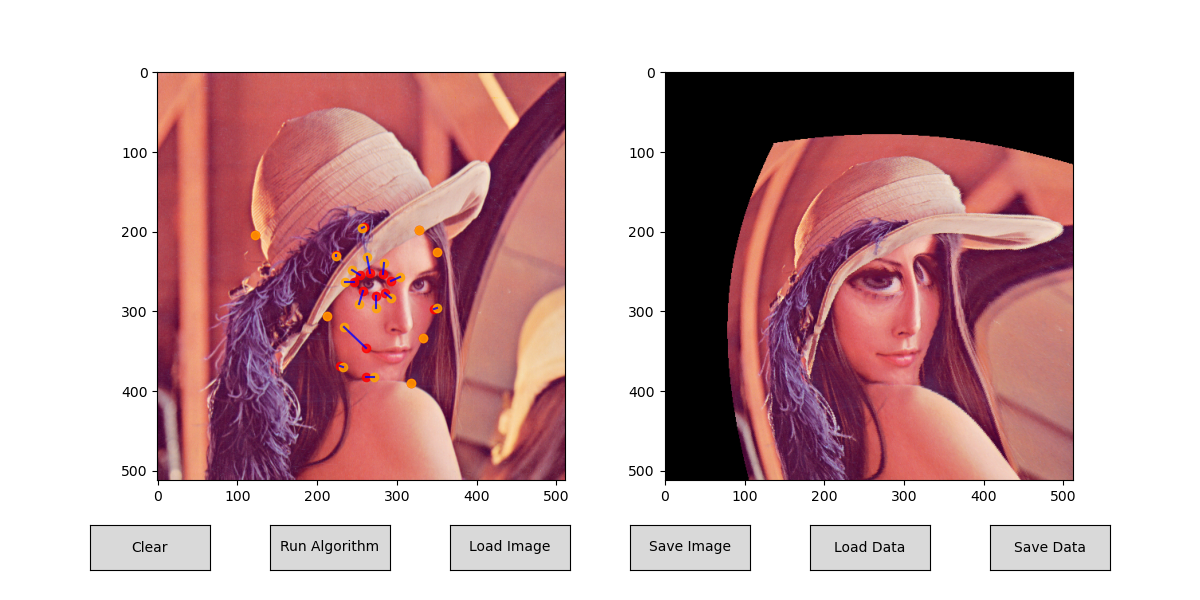
\includegraphics[width=0.6\textwidth]{Figures/Figure_iw.png}
		    	\caption{Image warping example}
		    	\label{fig:image-warping}
	\end{figure}
\end{solution}

\begin{exercise}
	\bf Bias-Variance Trade-off
\end{exercise}

\begin{solution}
	Since \(\mathbf{w}^T \bm{\phi}(x_n) \in \mathbb{R}\), we have 
	\[
	\mathbf{w}^T \bm{\phi}(x_n) = \bm{\phi}(x_n)^T \mathbf{w}.
	\]
	Therefore, the loss function can be expressed as 
	\[
	L^{(l)}(\mathbf{w}) = \frac{1}{2} \sum_{n=1}^N \left( y^{(l)}_n - \mathbf{w}^T \bm{\phi}(x_n) \right)^2 + \frac{\lambda}{2} \mathbf{w}^T \mathbf{w}.
	\]
	This can be rewritten as 
	\[
	L^{(l)}(\mathbf{w}) = \frac{1}{2} \sum_{n=1}^N \left( y^{(l)}_n - \bm{\phi}(x_n)^T \mathbf{w} \right)^2 + \frac{\lambda}{2} \mathbf{w}^T \mathbf{w} = \frac{1}{2} \|\mathbf{y}^{(l)} - \bm\Phi \mathbf{w}\|^2_2 + \frac{\lambda}{2} \mathbf{w}^T \mathbf{w},
	\]
	where \(\bm\Phi = \begin{pmatrix} \bm\phi(x_1) \\ \bm\phi(x_2) \\ \vdots \\ \bm\phi(x_n) \end{pmatrix}\).
	Taking the gradient, we find 
	\[
	\frac{\partial L^{(l)}(\mathbf{w})}{\partial \mathbf{w}} = -\bm\Phi^T (\mathbf{y}^{(l)} - \bm\Phi \mathbf{w}).
	\]
	Setting the gradient to zero, we obtain 
	\[
	\hat{\mathbf{w}}^{(l)} = \left( \bm\Phi^T \bm\Phi + \lambda \mathbf{I} \right)^{-1} \bm\Phi^T \mathbf{y}^{(l)}.
	\]
	\newline\newline
	2.  The image is shown below.
		\begin{figure}[htbp]
				\centering
			    	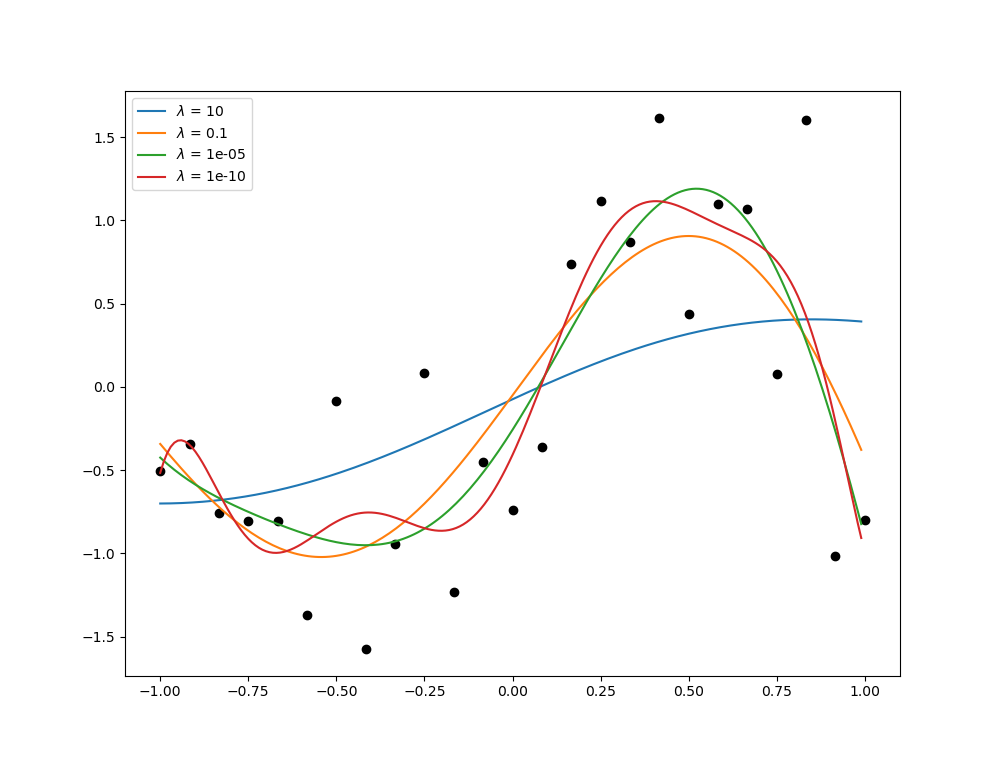
\includegraphics[width=0.6\textwidth]{Figures/Figure_bv_1.png}
			    	\caption{Fitting}
			    	\label{fig:bv_1}
		\end{figure} 
	\newpage
	3.  The image is shown below.
		\begin{figure}[htbp]
				\centering
			    	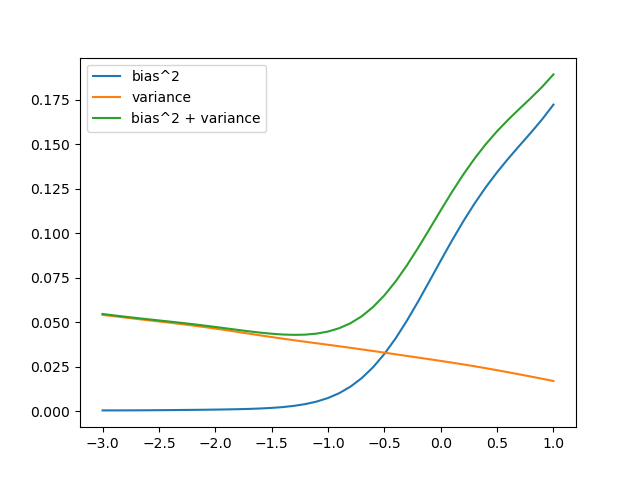
\includegraphics[width=0.6\textwidth]{Figures/Figure_bv_2.png}
			    	\caption{BV-tradeoff}
			    	\label{fig:bv_2}
		\end{figure} 
\end{solution}

\end{document}